\documentclass[b0paper,portrait,fontscale=0.24]{baposter}
\usepackage{amsmath}
\usepackage{amssymb}
\usepackage{relsize}
\usepackage{url}
\usepackage{enumitem}
% \usepackage{natbib}
\usepackage{braket}
\usepackage{multicol}
\usepackage[version=3]{mhchem}
\usepackage{microtype}

\usepackage{amsmath}
\usepackage{amssymb}
\usepackage{amsfonts}
\usepackage{amsopn}
\usepackage{braket}
\usepackage{bbm}
\usepackage{dsfont}
\usepackage{kpfonts}
% \usepackage{mathabx}

\parindent=0cm


% Various new commands that ease typesetting math even further
% \newcommand{\assign}{\ensuremath{\coloneq}}
% \newcommand{\rassign}{\ensuremath{\eqcolon}}
\newcommand{\assign}{\ensuremath{:=}}
\newcommand{\rassign}{\ensuremath{=:}}

\newcommand{\of}[1]{\ensuremath{\left( #1 \right)}}
\newcommand{\ofs}[1]{\ensuremath{\left( #1 \right)}}

\newcommand{\norm}[1]{\ensuremath{\| #1 \|}}

\newcommand{\tmop}[1]{\ensuremath{\operatorname{#1}}}

\newcommand{\id}{\ensuremath{\mathds{1}}}
% \newcommand{\id}{\ensuremath{I}}


\newcommand{\conj}[1]{\ensuremath{\overline{#1}}}

\newcommand{\T}{\ensuremath{{}^{\textnormal{T}}}}
\newcommand{\herm}{\ensuremath{{}^{\textnormal{H}}}}

\newcommand{\ft}[1]{\ensuremath{\mathcal{F}\left(#1\right)}}
\newcommand{\ift}[1]{\ensuremath{\mathcal{F}^{-1}\left(#1\right)}}

\newcommand{\fft}[1]{\ensuremath{\mathtt{FFT}\left(#1\right)}}
\newcommand{\ifft}[1]{\ensuremath{\mathtt{IFFT}\left(#1\right)}}

\newcommand{\dotp}[2]{\ensuremath{\langle #1 , #2 \rangle}}

\newcommand{\bigO}[1]{\ensuremath{\mathcal{O}\left( #1 \right)}}

\newcommand{\mat}[1]{\ensuremath{\mathbf{#1}}}

% multi-indices
\newcommand{\mindex}[1]{\ensuremath{\underline{#1}}}

\newcommand{\laplace}{\ensuremath{\operatorname{\Delta}}}

% EOF


% Global Settings
\graphicspath{{fig/}}

\definecolor{bordercol}{RGB}{40,40,40}
\definecolor{headercol1}{RGB}{186,215,230}
\definecolor{headercol2}{RGB}{186,215,230}
\definecolor{headerfontcol}{RGB}{0,0,0}
\definecolor{boxcolor}{RGB}{186,215,230}

% Save space in lists.
\setlist{nolistsep,leftmargin=*}
\setitemize{nolistsep,leftmargin=*}

% \newenvironment{itemize*}%
% {\begin{itemize}%
%   \setlength{\itemsep}{0pt}%
%   \setlength{\parskip}{0pt}%
%   \setlength{\parsep}{0pt}%
%   \setlength{\listparindent}{0pt}}%
%   {\end{itemize}}

\newenvironment{shrinkeq}[1]
{ \bgroup
  \addtolength\abovedisplayshortskip{#1}
  \addtolength\abovedisplayskip{#1}
  \addtolength\belowdisplayshortskip{#1}
  \addtolength\belowdisplayskip{#1}}
{\egroup\ignorespacesafterend}

\newcommand{\alert}[1]{{\red {#1}}}
\renewcommand{\imath}{\ensuremath{i}}


\begin{document}

% Setting Background Image
\background{
  \begin{tikzpicture}[remember picture,overlay]%
    \draw (current page.north west)+(-2em,2em) node[anchor=north west]
    {
\includegraphics[height=1.1\textheight]{background}};
  \end{tikzpicture}
}

% General Poster Settings
\begin{poster}{
    grid=false,
    eyecatcher=true,
    borderColor=bordercol,
    headerColorOne=headercol1,
    headerColorTwo=headercol2,
    headerFontColor=headerfontcol,
    linewidth=1pt,
    headerborder=closed,
    headershape=smallrounded,
    headerfont=\Large\sf\bf,
    textborder=roundedsmall,
    background=user,
    boxColorOne=boxcolor,
    boxshade=plain,
    columns=3
  }
  %
  {
    % The template centers the title *only* when using eyecatcher.
    % Eye Catcher, empty if option 'eyecatcher' is 'false'.
  }
  % Title
  {
    {\sf\bf
      Highly Oscillatory Integrals in Context}
    \vspace{4pt}
    {\sf\bf
      of Semiclassical Wavepackets
    }
  }
  % Authors
  {
    \vspace{2pt}
    \textit{Raoul Bourquin} and Vasile Gradinaru\\
    {\small raoul.bourquin@sam.math.ethz.ch,
      vasile.gradinaru@math.ethz.ch,
    }
  }
  % Logo
  {
    \begin{minipage}{14em}
      
\includegraphics[scale=0.65]{ETH_Logo} \\
      
\includegraphics[scale=0.5]{SAM_Logo}
    \end{minipage}
  }


  \headerbox{Semiclassical Wavepackets}{name=wavepackets,span=1,column=0,row=0}{
    We start from a Gaussian wavepacket:
    \begin{shrinkeq}{-1ex}
      \begin{equation*}
        \begin{split}
          & \phi_{\vec{0}}^{\hbar} [\vec{q},\vec{p},\mat{Q},\mat{P}](\vec{x})
          = (\pi\hbar)^{-\frac{d}{4}} (\det \mat{Q})^{-\frac{1}{2}} \,\times \\
          & \exp\left(\frac{i}{2\hbar}
            % \left(\vec{x}-\vec{q}\right)\T \mat{P}\mat{Q}\inv \left(\vec{x}-\vec{q}\right)
            \dotp{\vec{x}-\vec{q}}{\mat{P}\mat{Q}\inv \left(\vec{x}-\vec{q}\right)}
            + \frac{i}{\hbar}
            % \vec{p}\T \left(\vec{x}-\vec{q}\right)
            \dotp{\vec{p}}{\vec{x}-\vec{q}}
          \right)
        \end{split}
      \end{equation*}
    \end{shrinkeq}
    where the vectors $\vec{q}\in \mathbb{R}^d$ and $\vec{p}\in \mathbb{R}^d$
    represent the position and momentum, respectively, and $\mat{Q}$ and $\mat{P}$
    are complex $d\times d$ matrices. Raising and lowering operators $\mathcal{R}$
    and $\mathcal{L}$ then produce all higher order wavepackets $\phi_{\vec{k}}$
    for multi-indices $\vec{k} = (k_1,\dots,k_d)$ with non-negative integers $k_j$.
    The set of all parameters denoted by $\Pi := \{\vec{q},\vec{p},\mat{Q},\mat{P}\}$
    determines the \emph{family} of a wavepacket:
    \begin{shrinkeq}{-1ex}
      \begin{equation*}
        \Psi[\Pi](x,t) := \sum_{\vec{k} \in \mathfrak{K}} c_{\vec{k}}(t) \phi_{\vec{k}}[\Pi](x)
      \end{equation*}
    \end{shrinkeq}
    The set $\{\phi_{\vec{k}}\}_{\vec{k}\in\mathfrak{K}}$ forms a complete basis of $L^{2}$.
    \begin{minipage}[c]{\linewidth}
      \begin{center}
        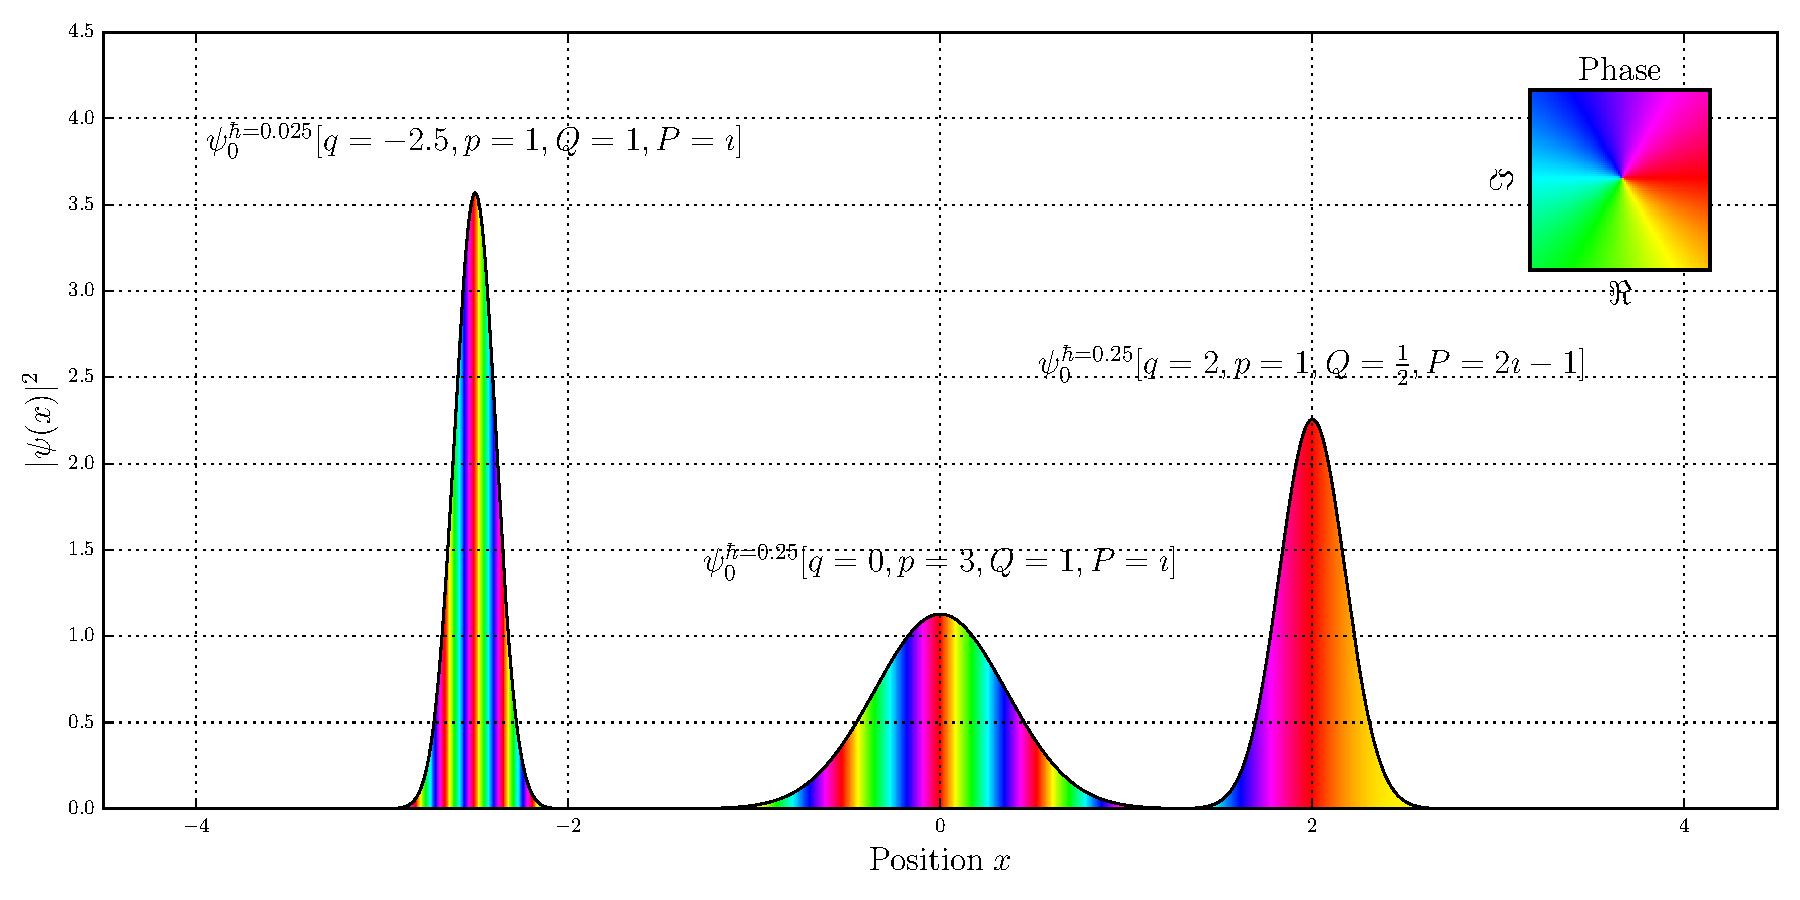
\includegraphics[width=\textwidth]{wavepackets.pdf}
      \end{center}
    \end{minipage}
  }


  \headerbox{Problem statement}{name=problem,span=1,column=0,row=0,below=wavepackets}{
    Our goal is to compute \emph{autocorrelations} like:
    \begin{shrinkeq}{-1ex}
      \begin{equation*}
        I = \Braket{\Psi[\Pi] | \Psi[\Pi^{\prime}]}
        = \idotsint_{\mathbb{R}^{d}} \conj{\Psi[\Pi]} \Psi[\Pi^{\prime}] \mathrm{d}\vec{x}
      \end{equation*}
    \end{shrinkeq}
    Computing that integral by standard numerical quadrature schemes turns out to be
    very difficult.
    In the most interesting cases where $\Pi \approx \Pi^{\prime}$ holds, Gaussian
    quadrature introduces huge errors and hence spurious correlations.
    \begin{minipage}[t]{\linewidth}
      \begin{minipage}[t]{0.49\linewidth}
        % \begin{minipage}[t]{\linewidth}
        \begin{center}
          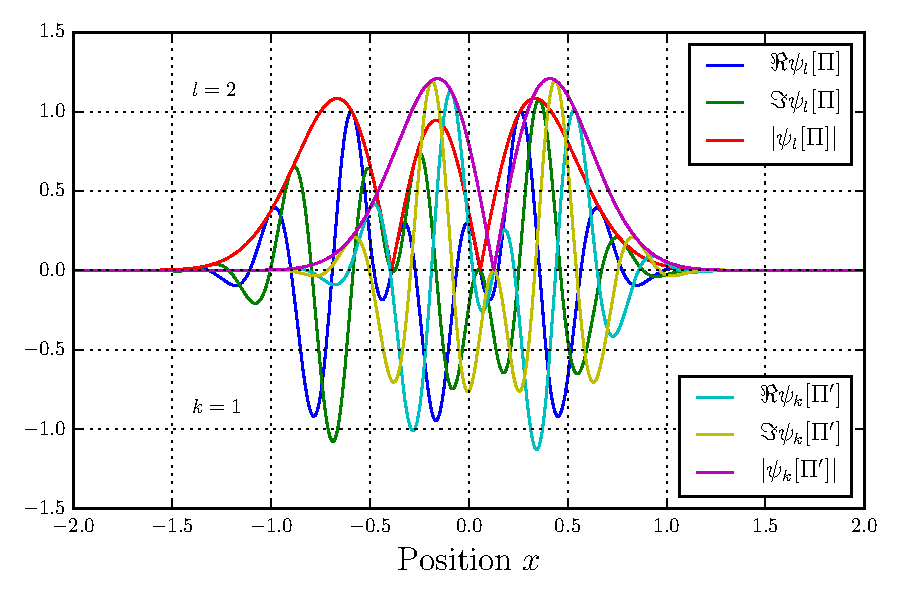
\includegraphics[width=\textwidth]{overlap_wavepackets.pdf}
        \end{center}
      \end{minipage}
      \hfill
      \begin{minipage}[t]{0.49\linewidth}
        % \begin{minipage}[t]{\linewidth}
        \begin{center}
          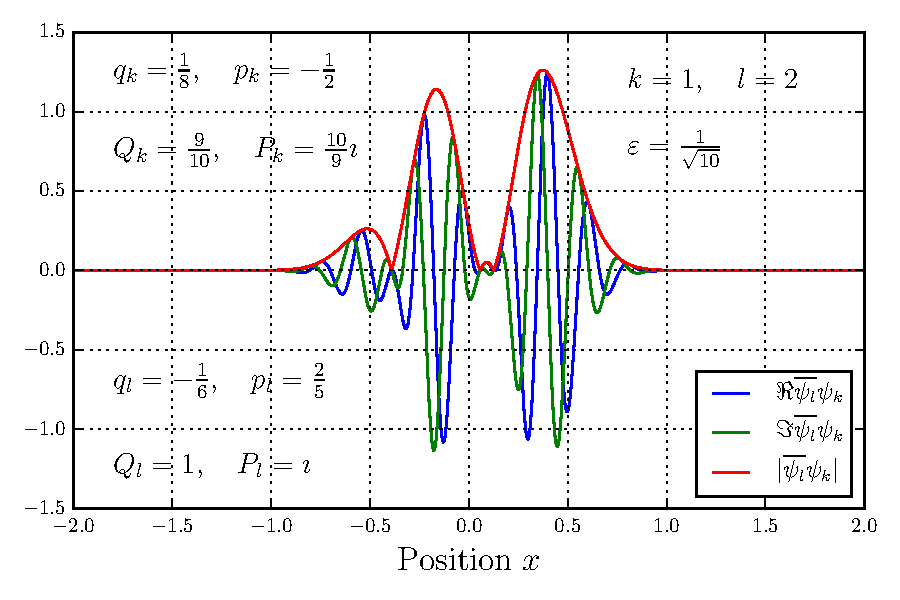
\includegraphics[width=\textwidth]{overlap_integrand.pdf}
        \end{center}
      \end{minipage}
    \end{minipage}
    \vspace{-0.4cm}
  }


  \headerbox{Conclusions and Limitations}{name=limitations,span=1,column=0,row=0,below=problem}{
    The most important conclusions and limitations for this
    \emph{numerical steepest descent} technique are:
    \begin{itemize}
    \item Works better for larger $\omega$ hence for smaller $\varepsilon$
    \item Works very well for $\Pi \approx \Pi^{\prime}$ (interesting case)
    \item Still need full tensor grid of quadrature nodes,
      but much less nodes in each direction
    \item In higher dimensions: use Smolyak sparse grids
    \item Envelope $f$ is assumed to have no poles in $\mathbb{C}^{d}$
    \item Unsuitable for $\Braket{\Psi|V|\Psi}$ \& non-polynomial $V$
    \end{itemize}
  }


  \headerbox{Numerical Steepest Descent}{name=nsd,span=2,column=1,row=0}{
    \begin{minipage}[t]{\linewidth}
      \begin{minipage}[t]{0.69\linewidth}
        The integral
        $I = \int_{a}^{b} f(x) \exp\left(\imath \omega g(x)\right) \mathrm{d}x$
        is highly oscillatory with frequency $\omega \in \mathbb{R}^{+}$.
        \textbf{Idea}: transform the integrand, such that it is no longer
        oscillatory but rather exponentially decaying. \cite{HV_hoq}
        \textbf{Mean}: find a coordinate transform such that the \emph{real}
        part of $g$ is constant.
        \begin{itemize}
        \item Decompose integrand into an oscillator $g(x)$ and an envelope $f(x)$
        \item Find all the stationary points $\{x_{j}^{*}\}_{j}$ from the gradient:
          $\nabla_{x} \, g(x) = 0$
        \item Set up the path equation $g(h_{\xi}(\tau))=g(\xi) + \imath \tau$
          for each $\xi := x_{j}^{*}$
        \item Compute all paths $h_{\xi}(\tau)$ with $\xi \in \{a,b\} \cup \{x_{j}^{*}\}_{j}$ and $\tau \in \mathbb{R}_{0}^{+}$
        \item Apply the transformations $x \mapsto h_{\xi}(\tau)$ and obtain a bunch of integrals
        \end{itemize}
        End up with:
        \begin{shrinkeq}{-2ex}
          \begin{equation*}
            I = e^{\imath\omega} J[a]
            + \sum_{j} \left(J[x_{j,+}^{*}] - J[x_{j,-}^{*}]\right)
            - e^{\imath\omega} J[b]
          \end{equation*}
        \end{shrinkeq}
        where
        \begin{shrinkeq}{-0ex}
          \begin{equation*}
            J[\xi] := \int_{0}^{\infty}
            f(h_{\xi}(\tau)) \,
            h_{\xi}^{\prime}(\tau) \,
            e^{-\omega \tau} \,
            \mathrm{d}\tau
          \end{equation*}
        \end{shrinkeq}
      \end{minipage}
      \hfill
      \begin{minipage}[t]{0.29\linewidth}
        \vspace{-0.4cm}
        \begin{center}
          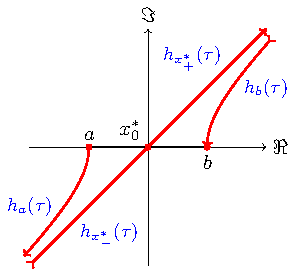
\includegraphics[width=\textwidth,height=\textwidth]{nsd_path_figure.pdf}
        \end{center}
        \vspace{-0.4cm}
        Oscillator $g(x)=x^{2}$ with single stationary point $x^{*}_{0}=0$.
        Integration paths $h_{a}(\tau)$, $h_{x^{*}_{0},-}(\tau)$,
        $h_{x^{*}_{0},+}(\tau)$ and $h_{b}(\tau)$.
      \end{minipage}
    \end{minipage}
    Finally, approximate these integrals $J$ by a suitable quadrature rule
    along the complex path. In higher dimensions this becomes a much more
    involved iterative scheme but the basic principles stay the same.
  }


  \headerbox{Numerical Steepest Descent for Wavepackets}{name=nsdforwp,span=2,column=1,row=0,below=nsd}{
    \begin{minipage}[t]{\linewidth}
      \begin{minipage}[t]{0.57\linewidth}
        For wavepackets
        $\phi_{\vec{k}} \!\sim\! p_{\vec{k}}\left(\vec{x}\right)\exp\!\left(\frac{\imath}{\varepsilon^2}g_{\vec{k}}\!\left(\vec{x}\right)\right)$
        we have \cite{BG_nsd}:
        \begin{shrinkeq}{-1ex}
          \begin{equation*}
            \Braket{\phi_{\vec{l}} | \phi_{\vec{k}}}
            \sim \int_{\mathbb{R}^{d}}
            \conj{p_{\vec{l}}(\vec{x})} p_{\vec{k}}(\vec{x})
            \exp\left(
              \frac{\imath}{\varepsilon^{2}}
              \left(
                g_{\vec{k}}(\vec{x}) - \conj{g_{\vec{l}}(\vec{x})}
              \right)
            \right)
            \mathrm{d}\vec{x}
          \end{equation*}
        \end{shrinkeq}
        \begin{itemize}
        \item Envelope $f := \conj{p_{\vec{l}}} p_{\vec{k}}$ is a polynomial and hence pole-free
        \item Quadratic oscillator
          $g(\vec{x}) := g_{\vec{k}} - \conj{g_{\vec{l}}} = \vec{x}\H \mat{A} \vec{x} + \vec{b}\T\vec{x} + c$
        \item $\mat{A}$ is \emph{not} Hermitian but $\Re\mat{A}$ and $\Im\mat{A}$
          are \emph{symmetric}
          % \item Use affine transform to remove linear and constant terms from $g(\vec{x})$
        \item \emph{Schur decomposition} $\mat{A} = \mat{U}\H \mat{T} \mat{U}$
          % of $\mat{A}$ to obtain a new oscillator
          yields $\tilde{g}(\tilde{\vec{x}}) = \tilde{\vec{x}}\H \mat{T} \tilde{\vec{x}}$
          % with upper triangular matrix $\mat{T}$ and unitary $\mat{U}$
        \item Infinite interval $(-\infty, \infty)^{d}$, boundary terms disappear
        \item Single point $x^{*} \in \mathbb{C}^{d}$ is computed from a linear system
        \item Path equations are solvable by closed form for all $h_{\xi}(\vec{\tau})$
        \item Pairs of paths lie on a straight line, can be glued together
        \item Integrand is $a(\vec{\tau})\,e^{(-\vec{\tau}\cdot \vec{\tau})}$,
          use \emph{Gauss-Hermite quadrature}
        \end{itemize}
        Contour levels and zeros (blue) of $|\conj{\phi_{\vec{l}}} \phi_{\vec{k}}|$,
        Gradient field and zeros of $|g|$ (yellow),
        Path of steepest descent with 9 Gauss Hermite quadrature nodes (red),
        in complex plane.
      \end{minipage}
      \hfill
      \begin{minipage}[t]{0.42\linewidth}
        \vspace{-0.3cm}
        \begin{center}
          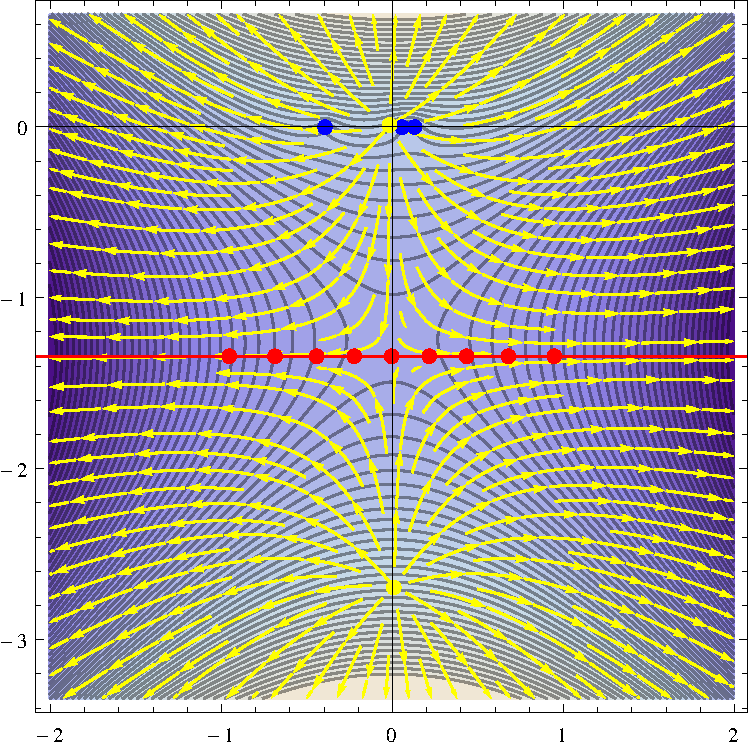
\includegraphics[width=\textwidth,height=\textwidth]{stationary_point_example.pdf}
        \end{center}
        % \vspace{-0.35cm}
      \end{minipage}
    \end{minipage}
    % In $d$ dimensions we get a complicated but systematic procedure for computing
    % all the paths iteratively, one variable at a time.
    % Finally we are left with $d$ straight line paths attached to the
    % stationary point.
  }


  \headerbox{Experiments and Convergence Results}{name=results,span=2,column=1,row=0,below=nsdforwp}{
    \begin{minipage}[t]{\linewidth}
      \begin{minipage}[t]{0.49\linewidth}
        \begin{center}
          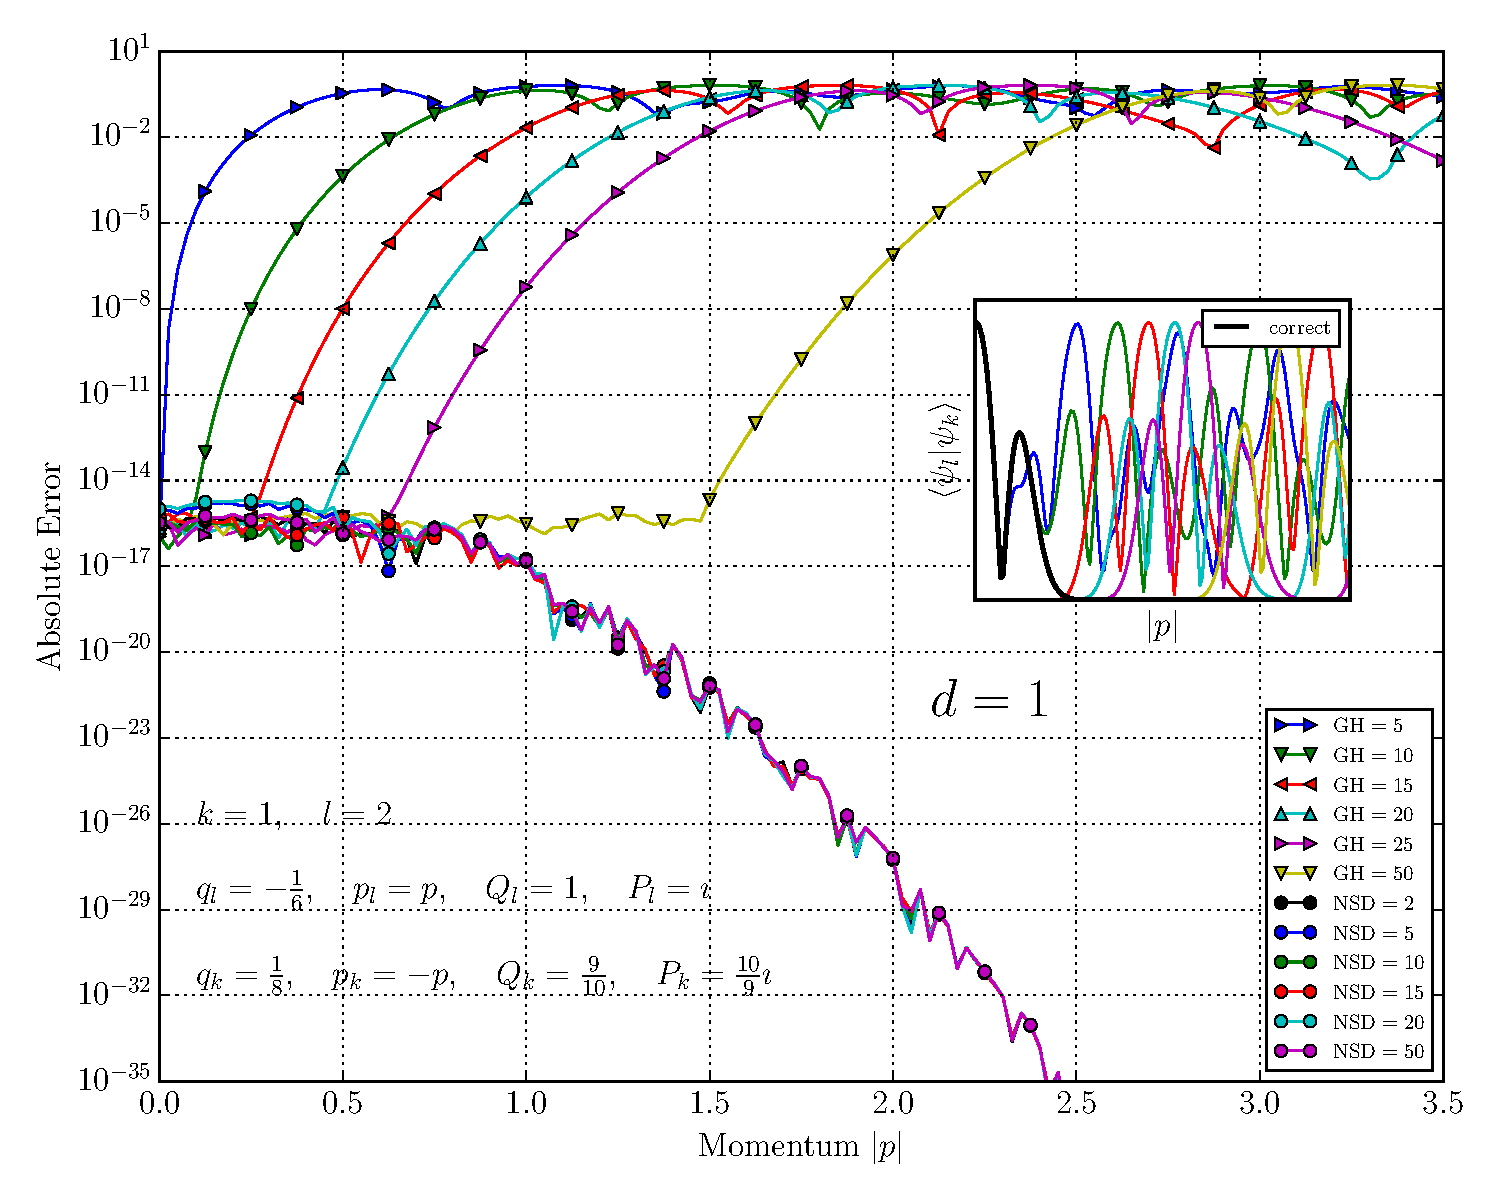
\includegraphics[width=\textwidth]{conv_momentum.pdf}
        \end{center}
      \end{minipage}
      \begin{minipage}[t]{0.49\linewidth}
        \begin{center}
          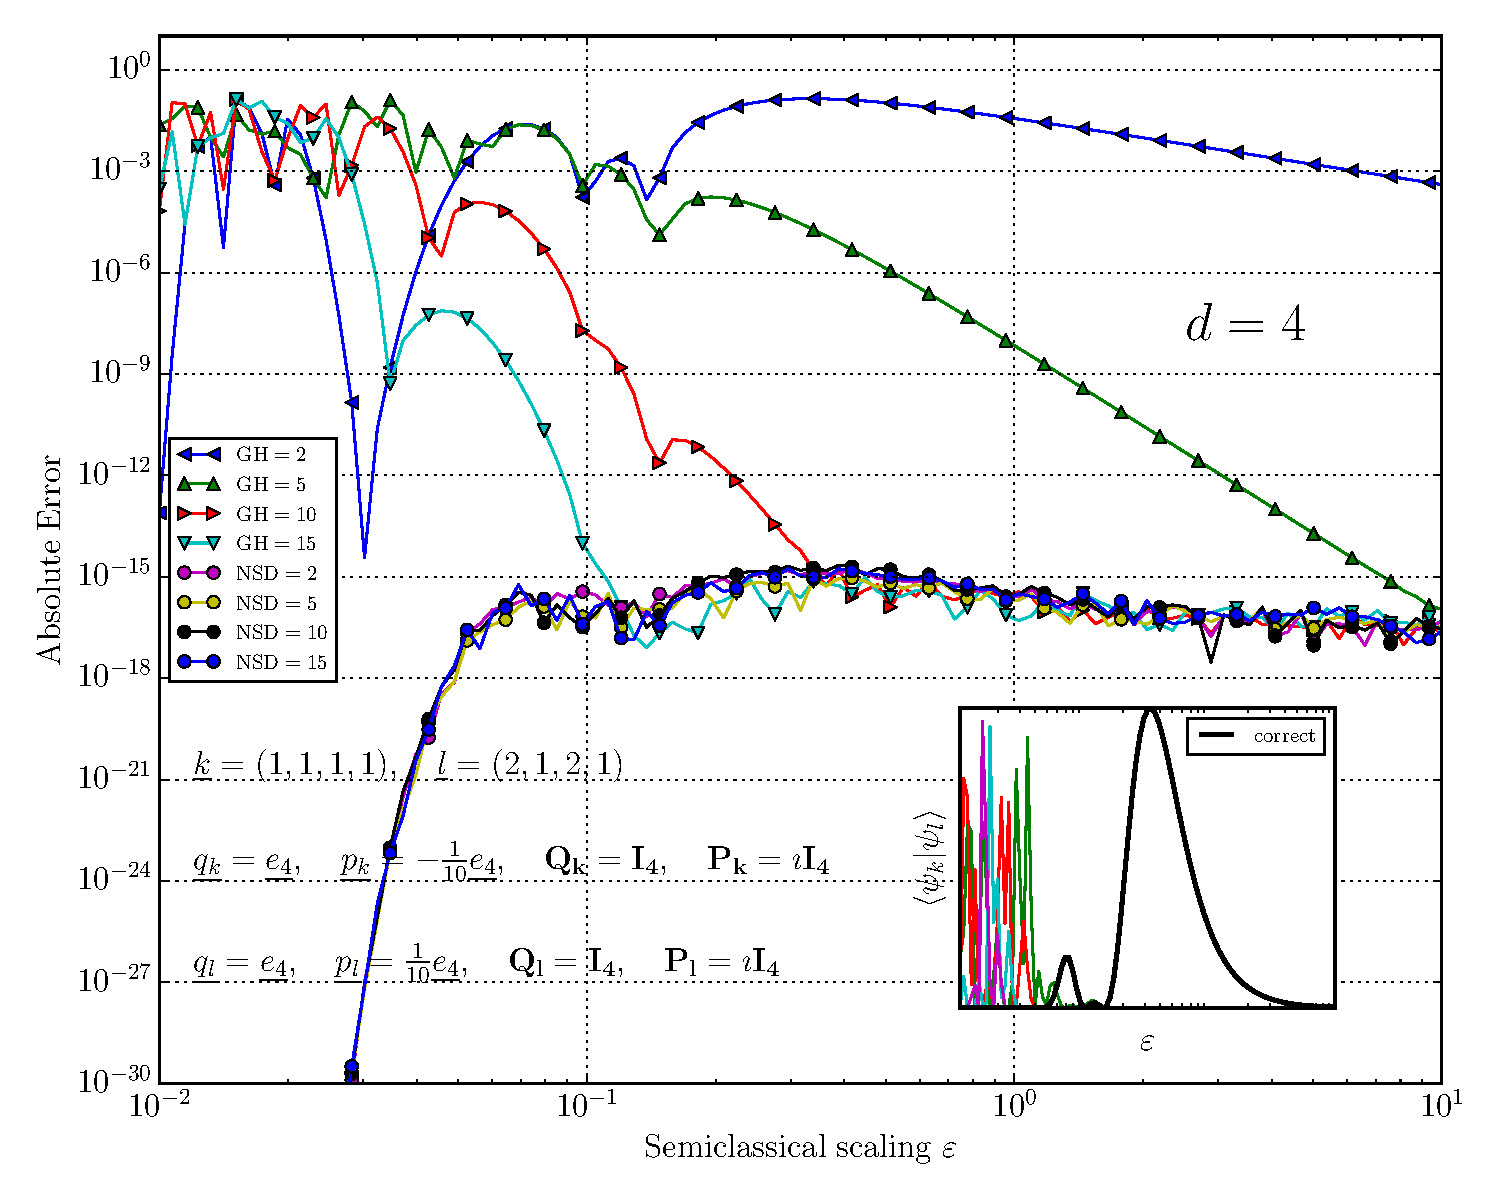
\includegraphics[width=\textwidth]{conv_eps.pdf}
        \end{center}
      \end{minipage}
      Experiments showing the convergence with increasing momentum $\vec{p}$
      and decreasing semiclassical parameter $\varepsilon$. The method of steepest descent
      performs very well compared to classical quadrature.
    \end{minipage}
  }


  \headerbox{Application to \ce{Hg2}}{name=application,span=2,column=1,row=0,below=results,above=bottom}{
    \begin{minipage}[t]{\linewidth}
      \begin{minipage}[t]{0.56\linewidth}
        We study the time-dependent Schr\"odinger equation
        with a wavepacket $\Psi$ propagating in the Morse potential $V$.
        The potential was fit to experimental data and the semiclassical
        parameter $\varepsilon$ matches the dynamics of mercury.
        \\
        \begin{minipage}[c]{0.49\linewidth}
          \begin{center}
            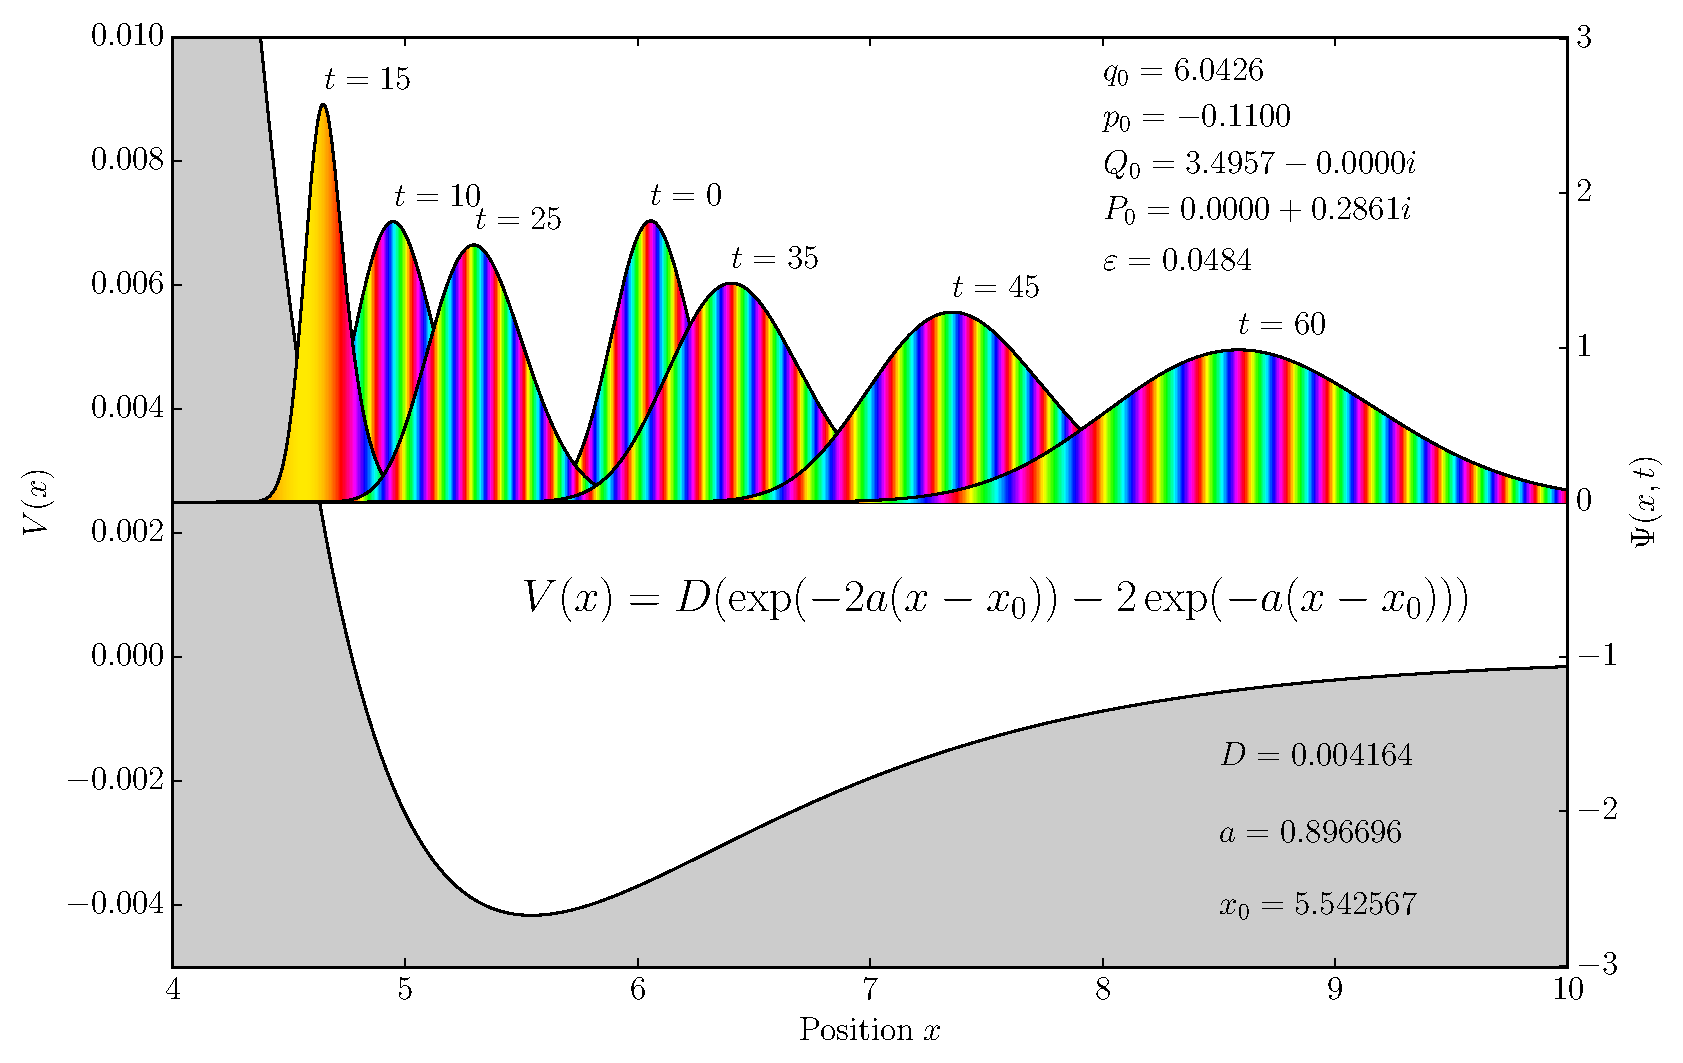
\includegraphics[width=1.0\textwidth]{hg_morse_wps.pdf}
          \end{center}
        \end{minipage}
        \begin{minipage}[c]{0.49\linewidth}
          Gauss Hermite quadrature with any number of nodes
          shows spurious autocorrelations.
          Using the steepest descent transformation gives correct
          results and requires a smaller number of nodes.
        \end{minipage}
      \end{minipage}
      \hfill
      \begin{minipage}[t]{0.42\linewidth}
        \vspace{-0.3cm}
        \begin{center}
          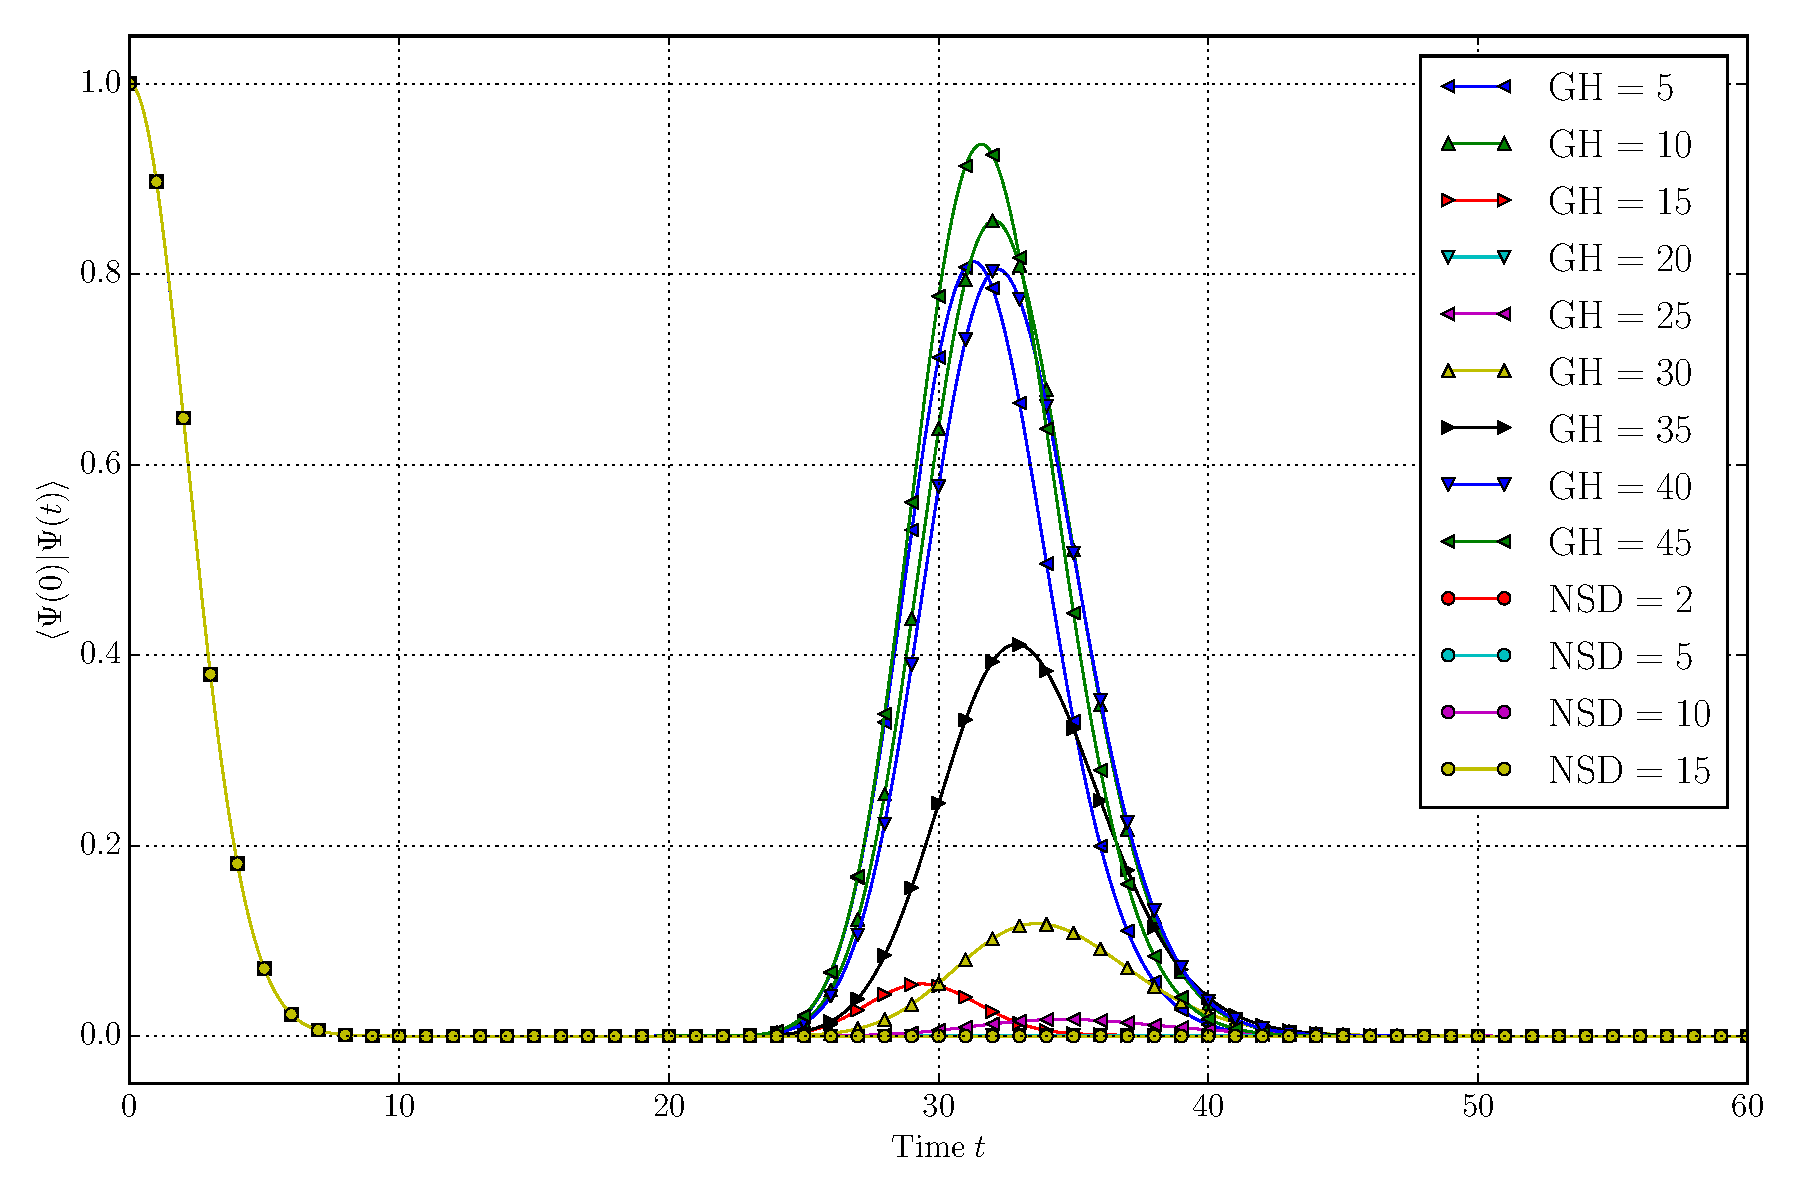
\includegraphics[width=\textwidth]{ac_mercurial_morse.pdf}
        \end{center}
      \end{minipage}
    \end{minipage}
  }


  \headerbox{References}{name=references,column=0,below=limitations}{
    \smaller
    \vspace{-1.em}
    \renewcommand\refname{}
    \bibliographystyle{plain}
    \bibliography{nsd,wp,own}
  }


  \headerbox{Source Code}{name=sourcecode,column=0,below=references,above=bottom}{
    \smaller
    \vspace{-1.em}
    \noindent
    \begin{minipage}{\linewidth}
      \begin{minipage}[c]{0.80\linewidth}
        Python code for semiclassical wavepackets:\\
        \url{https://github.com/raoulbq/WaveBlocksND}
      \end{minipage}\hfill
      \begin{minipage}[c]{0.20\linewidth}
        \hfill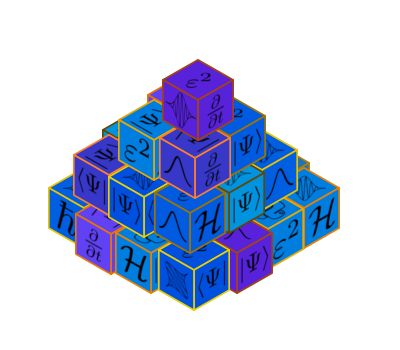
\includegraphics[width=\linewidth]{waveblocks}
      \end{minipage}
    \end{minipage}
    \vspace{-1.em}
  }


\end{poster}
\end{document}


%%% Local Variables:
%%% mode: latex
%%% TeX-PDF-mode: t
%%% End:
